\documentclass{article}
\usepackage[backend=biber]{biblatex}
\usepackage{graphicx}
\usepackage[]{hyperref}
\usepackage{booktabs}
\addbibresource{bibliography.bib}

\author{Anthony Steven Luna Gonzales, Roberto Giusto, Giulia Barbero}
\title{Turbina ad alta temperatura}

\begin{document}
    \maketitle
    \begin{center}
        
\includegraphics[width=0.9\textwidth]{Sources/polito_logo.png}\linebreak\newline
       \textbf{\textit{Materiali per applicazioni aerospaziali}}\linebreak\newline
        \textit{Gruppo di lavoro n. xx}\linebreak\newline
        \textit{Anno accademico 2020/2021}
    \end{center}

    \newpage
    \section{Introduzione}
    I turbomotori assiali aeronautici possono essere suddivisi, generalmente, in tre macrosezioni
    fondamentali: compressore, camera di combustione e turbina.\\
    \begin{center}
        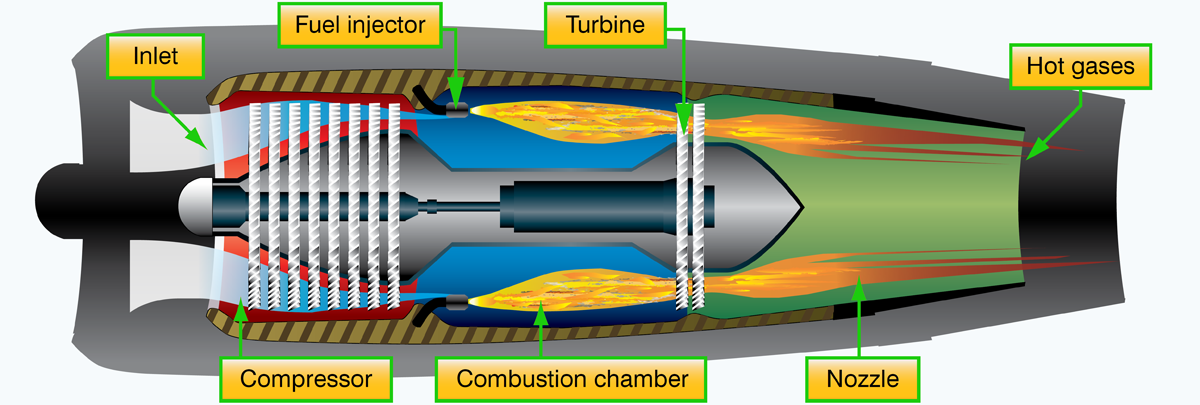
\includegraphics[width=0.8\textwidth]{Sources/turbojet.png}\\
        \textit{Fig.1 }: Schema generale di un motore turbojet \autocite*{turbojet} 
    \end{center}
    Un \textit{inlet} favorisce l'afflusso di aria esterna al \textit{compressore}, il quale
    la comprime in un volume nettamente inferiore, attraverso vari stadi alternati di pale rotoriche-statoriche.\\
    L'aria fortemente compressa viene poi miscelata con il carburante iniettato in \textit{camera di combustione},
    in una determinata proporzione (dipendente da vari fattori): la miscela viene quindi combusta, seguendo le trasformazioni di
    un preciso ciclo termodinamico (ogni motore ha la sua implementazione, ma i principi fondamentali sono gli stessi), causando un repentino
    aumento di pressione e temperatura.\\
    Successivamente, i gas combusti vengono espansi rapidamente dalla \textit{turbina} (la quale, inoltre, mette in rotazione l'albero di trasmissione), attraverso, in questo caso,
    vari stadi alternati di pale statoriche-rotoriche.\\
    Infine, i gas espansi vengono espulsi e accelerati attraverso un \textit{ugello}.\\
    Tutto il processo fornisce una spinta, secondo il principio di azione-reazione \autocite*{Aircr_engine_design}.\\ \\
    Le temperature e le sollecitazioni raggiunte dalle palette di turbina sono tipicamente in range estremi (in particolare per gli stadi ad alta pressione),
    al punto che la scelta dei materiali é sostanzialmente diversa da quella del compressore.\\
    In un moderno jet engine, si possono raggiungere temperature massime che eccedono i 1500 °C \autocite*{SciencePubGroup}, 
    senza contare le sollecitazioni meccaniche a cui sono sottoposte le pale HP, a causa di pressioni elevatissime,
    forze centrifughe per velocitá di migliaia di RPM e intense vibrazioni, nonché problemi di corrosione
    e reazioni chimiche indesiderate, favorite oltretutto dall'alta temperatura.\\
    
    \begin{center}
        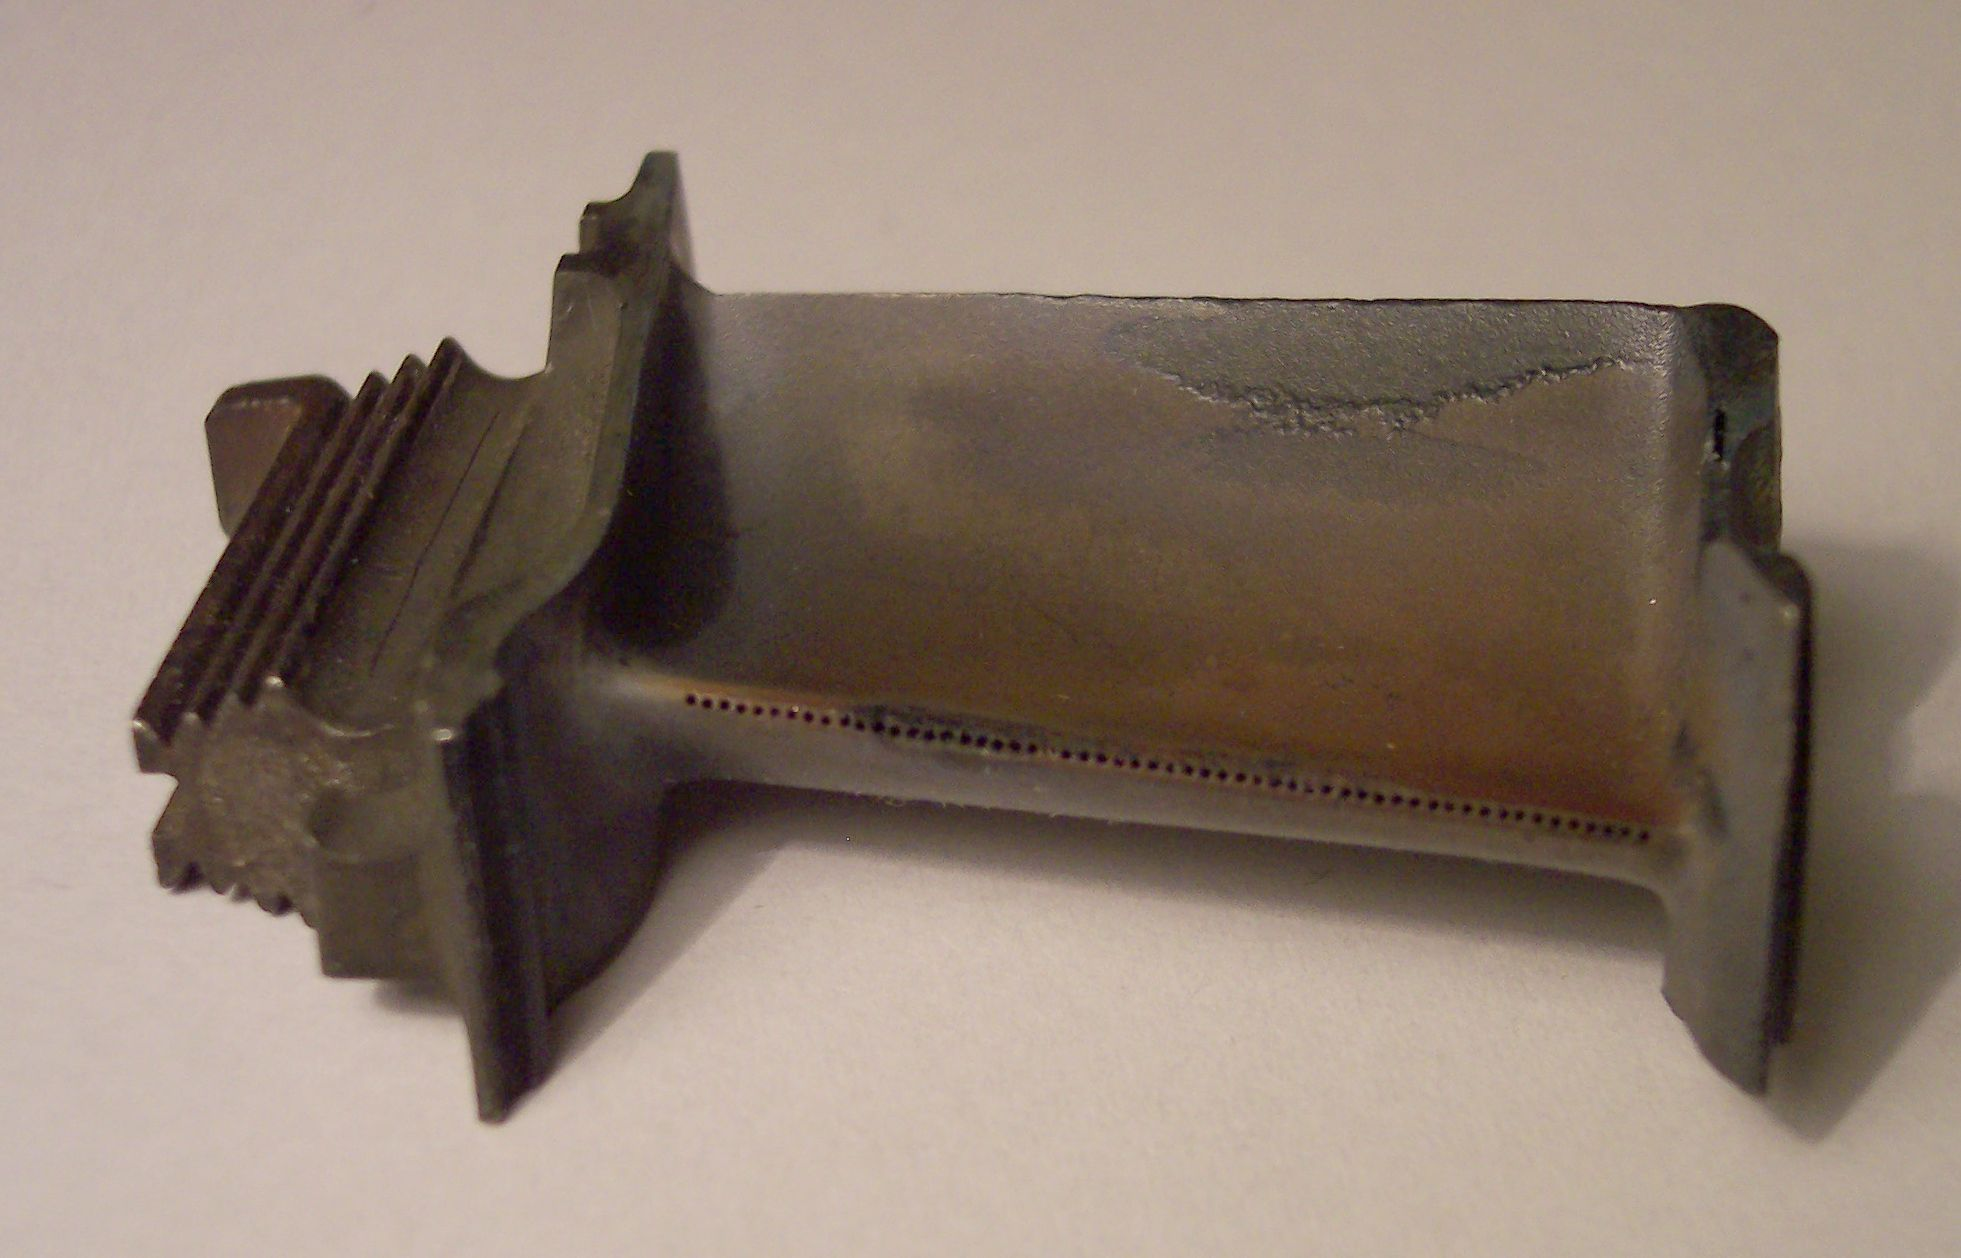
\includegraphics[width=\textwidth]{Sources/Turbinenschaufel_RB199.jpg}
        \textit{Fig.2 }: Gli effetti dell'ambiente operativo estremo su una paletta di turbina \autocite*{turbine_blade}
    \end{center}
    É necessario, dunque, scegliere un materiale (o una combinazione di piú materiali)
    in grado di sopportare, per il tempo di operativitá del componente, l'effetto
    simultaneo dell'elevatissima temperatura, dell'aggressivitá chimica e delle sollecitazioni meccaniche istantanee e cicliche,
     tenendo in considerazione, eventualmente, la possibilitá di un raffreddamento attivo.\\

    \pagebreak




    \section{Funzioni, obiettivi, vincoli}
        \begin{tabular}{l|r}
            \toprule
                \textbf{\textit{Funzione}}   & x\\
                \textbf{\textit{Obiettivi}}  & y\\ 
                \textbf{\textit{Vincoli}}    & z\\ 
            \bottomrule
        \end{tabular}   
    \section{Selezione dei materiali}
        \subsection{Stadio 1}
        \subsection{Stadio 2}
        \subsection{Stadio 3}
        \dots
        \subsection{Stadio N}
    \section{Conclusioni}
    
    \printbibliography
    
\end{document}
